% !TeX root = ../my-thesis.tex
\chapter{Grundlagen}
Laut des IT-Grundschutz-Kompendiums vom Bundesamt für Sicherheit in der Informationstechnik könne ein Benutzer aus Bequemlichkeit oder pragmatischen Gründen bewusst auf komplizierte und unhandliche Kryptomodule verzichten und Informationen stattdessen im Klartext übertragen. \cite{A1} Dies stellt ein hohes Sicherheitsrisiko für Unternehmen, aber auch Privatpersonen dar, da Benutzer nicht gewillt sind ihre Passwörter durch komplizierte Verfahren zu erzeugen und in regelmäßigen Abständen vollkommen randomisiert zu setzen. An neuartige Ansätze des Logins in nativen oder webbasierten Anwendungen stellen sich dadurch völlig neue Herausforderungen. So müssen neue Authentifizierungsmöglichkeiten nicht nur sicher sein, sondern auch komfortabel genutzt und bedient werden können, da sie sonst von den Endnutzern gemiedern oder umgangen werden. Wichtig ist eben auch, dass die breite Masse Zugriff auf die Ressourcen hat, die es zur Nutzung dieser Verfahren braucht. Man denke nur an die ganzen betrieblichen Passwörter, bei denen zum Monatsende nur eine Zahl an der letzten Stelle des Passwortes geändert wird. Laut einer Statistik von 2019, der "Global Data Risk Report From the Varonis Data Lab", gaben 38\% aller Nutzer an ein Passwort im Unternehmen zu nutzen, dass sie nicht (oder nur geringfügig) ändern. Außerdem wird laut dieser Statistik alle 364 Tage ein Data-Breach aufgrund von unsicheren Passwörtern in einem mittelständigen Unternehmen stattfinden. Die monatliche Ablaufzeit von Passwörtern in Unternehmen scheint also nicht ganz den Effekt zu erzielen, der ursprünglich damit geplant war, da die Arbeiter die Bequemlichkeit über die Sicherheit stellen.

\section{IT-Grundschutzkriterien}
Der IT-Grundschutz definiert den Schutzbedarf eines bestimmten Assets je nachdem welches Risiko bei Verletzung der Grundwerte Vertraulichkeit, Integrität und Verfügbarkeit entstehen [10]. Allgemein existieren folgende Schutzbedarfskategorien:
\begin{itemize} 
\item \textbf{normal} (Schadenauswirkungen begrenzt bis überschaubar)
\item \textbf{hoch} (Schadenauswirkungen könnten hoch bzw. beträchtlich sein)
\item \textbf{sehr hoch} (Schadensauswirkungen können ein existenziell bedrohliches Ausmaß annehmen
\end{itemize}
Bei dem Authentifikationsprototypen wird die Schadensauswirkung für alle nicht personenbezogenen Daten wohl im Bereich normal liegen, da schon im Aufbau darauf geachtet wird, dass nur so viele Daten vom User verwendet werden, wie zwingend notwendig. (Nach dem Need-To-Know Prinzip) Sollte die Webseite oder Teile der Webseite publiziert bzw. im Business - Umfeld genutzt werden, muss eine Neubewertung der Daten nach Vertraulichkeit, Integrität und Verfügbarkeit stattfinden. Vor allem muss darauf geachtet sein, dass Daten über Fingerabdrücke verschlüsselt und Passwörter im gehashten Zustand in Datenbanken persistiert werden. Bei Kompromittierung des Hauptrechners, welches die größte Bedrohung in diesem Szenario darstellen würde, droht ein Data Breach mit dem Angreifer diese Daten weiterverwenden können. Durch Verschlüsselungen durch Schlüssel, die nicht auf dem Hauptsystem (oben u.a als Hauptrechner benannt) liegen. Gleichzeitig sollten die genutzten Verfahren insgesamt mathematisch sicher sein, auf veraltete Verschlüsselungsverfahren ist zu verzichten. Dies gillt auch für Hashes wie MD5, die mittlerweile relativ akkurat durch sehr große vorgerechnete Tabellen erraten werden können. \newpage

Im Falle einer Kompromittierung besäße der Schutzbedarf der Daten innerhalb der Datenbank, welche nicht gehasht oder anderweitig verschlüsselt sind, die Kategorie 'sehr hoch'. Eine Kompromittierung kann für das Unternehmen einen Imageschaden sowie weitreichende juristische Klagen zur Folge haben. Damit sind bereits 2 der 7 aufgeführten Schadensszenarien durch den \ac{bsi} beschrieben. Je nach dem wie kompliziert die Ursprungsdaten sind und welcher Hashingalgorithmus in Kombination mit Salt und Pepper genutzt wurde, können vorallem Nutzerpassphrasen an die Öffentlichkeit gelangen und Angreifer können die Passwörter für andere Dienste nutzen. Die Wahrscheinlichkeit für diesen Schaden ist noch vergleichbar niedrig, weshalb die Schadensauswirkung hoch statt sehr hoch ist.

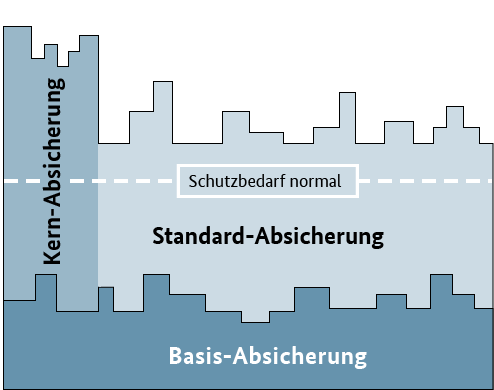
\includegraphics[width=15cm]{Abb_2_09_Varianten.png}

Der IT-Grundschutz definiert drei Arten der Absicherung. Die Basis-Absicherung ist relevant für Institutionen die einen Einstieg in den IT-Grundschutz suchen und relativ schnell alle relevanten Geschäftspozesse mit einfach umzusetzenden Basismaßnahmen sichern wollen. Die Kern-Absicherung konzentriert sich auf besonders wichtige Geschäftsprozesse und vertieft sich in die Sicherung dieser. Von einer Standard-Absicherung spricht man, wenn alle empfohlenen IT-Grundschutz-Vorgehensweisen durchgeführt werden. Sie beschreibt den allumfassenden Schutz der Prozesse und Bereiche der Institution, wie das Schaubild vom BSI verdeutlicht. [9] Bei dem Prototyp wird eine Basis-Absicherung nach BSI durchgeführt und darauf geachtet alle Datenschutzkriterien zu erfüllen. Dabei wird vor allem die Checkliste des IT-Grundschutzes zu Webservern und Webanwendungen betrachtet. Kriterien die nicht erfüllt werden konnten oder wurden, werden dokumentiert und im Fazit erläutert. Die Wahl der Basis-Absicherung begründet sich damit, das lokale Testdaten im Prototyp verarbeitet werden, für die kein bis nur ein sehr geringer Schutzbedarf besteht. Eine Kern-Absicherung käme nur in Frage, falls ein ganz bestimmter Prozess oder Asset des Prototyps geschützt werden müsste wie zum Beispiel der Zugriff auf die Datenbank durch den Prototypen, welche nicht der Fall ist. Insgesamt ist dieser Teil der Abschlussarbeit auch als Einstieg in den IT-Grundschutz zu verstehen, welcher laut BSI selbst die Basis-Absicherung als Empfehlung und zur Folge meiner Entscheidung hat und sich am Besten für vorhandene Zwecke eignet.

\section{FIDO2}
Diese Probleme sind den Menschen seit einigen Jahren bekannt und wurden vor allem mit Verfahren gelöst, die keine Passwörter (oder allgemein weissensbasierte Token) zur Authentifikation benötigen und diesen maximal als ersten Layer der Sicherheit anerkennen. Das Bekannteste Beispiel für einen Standart zur sicheren und bequemen Authentifikation im Internet findet man unter dem Schlüsselwort FIDO2. FIDO steht dabei für 'Fast Identity Online' (Schnelle Identität im Netz). Sie ist das Ergebnis einer Kooperation des \ac{w3c} und der FIDO Alliance. FIDO2 basiert auf vorhandenen Protokollen wie \ac{webauthn} für die Browser-Server-Kommunikation und CTAP für die Browser-Authenticator-Kommunikation. Auf der offiziellen Webseite der yubico, einem der Hauptentwickler und Publizierer des Vorgängerprotokolls \ac{u2f} wird die FIDO2 - \ac{u2f}, also die zwei Faktor Authentifizierung spezifiziert durch \ac{u2f} das immernoch im FIDO2 Protokoll beheimatet ist, wie folgt beschrieben: ''an open authentication standard that enables internet users to securely access any number of online services with one single security key [...]. FIDO2 is the latest generation of the \ac{u2f} protocol`` [5]. Während das Vorgänger - Protokoll \ac{u2f} von Google und Yubico ins Leben gerufen wurde, ist FIDO2 ein offener dezentraler Kommunikationsstandart für die passwortlose Kommunikation welches die Authentifizierung für sowohl Privatnutzer als auch Unternehmen beqeuem und gleichzeitig sicher machen soll. \\ \\
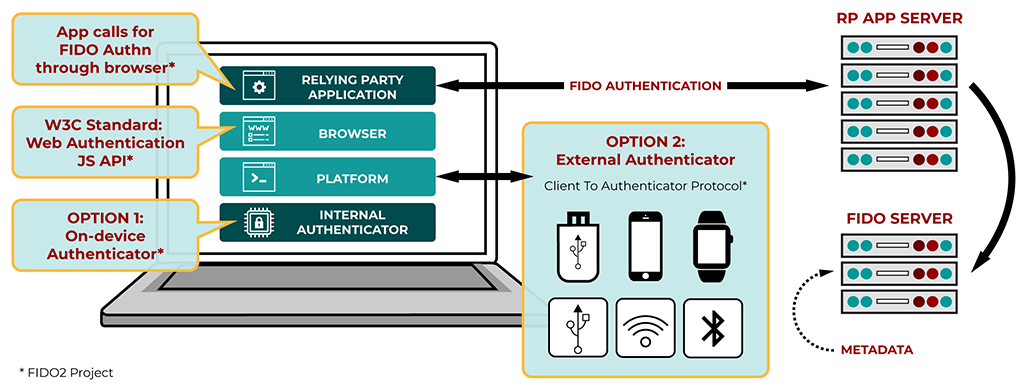
\includegraphics[width=15cm]{Graphics/FIDO2-Graphic-v2.png} \\
\\
Um die Sicherheit des Nutzers zu gewährleisten kombiniert FIDO2 die Methoden des UAF und des U2F. Bevor wie bei gängigen Zweifaktoren wie eines PINs oder sechsstelligen Schlüssels der Schlüsselaustausch stattfinden kann, muss der User der Anwendung oder des Dienstes eine lokale Verifikation durchführen. Diese soll sicherstellen, dass es sich bei der Person, die die Authentifikation durchführt und der Person, die den Schlüssel vorher registriert hat, um die selbe Person handelt. Diese Verifikation kann zum Beispiel ein Knopf auf einem USB - Stick sein, auf den der Web-Service wartet oder ein Fingerabdruck-Sensor - Bevor er die Challenge an den Nutzer (bzw. über dessen Browser dann an die Webseite) sendet. So lange also ein Angreifer keinen physischen Zugang zu diesem Gerät erhält, ist das Verfahren sicher. Sollte es doch vorkommen, dass der Angreifer sich Zugriff verschafft und den Knopf drückt, setzt die sozusagen zweite Phase der Authentifikation ein. Die Webseite sendet dem User eine Challenge, welche der User lokal mit seinem Schlüssel auf dem Computer lösen kann. Die Webseite erhält dann das Ergebnis und vergleicht dieses mit dem eigenen Ergebnis. Gibt es ein Match, sendet der Server der Webseite die zugehörige Response zur Challenge an den User zurück und lässt ihn passieren. Wie die Abbildung zeigt gibt es neben der externen Authentifikation durch Smart-Watch, USB- Stick oder Smartphone auch die Option der 'on-device-authentication'. Damit ist die Authentifizierung durch einen PIN oder einen eingebauten Fingerabdruck-Sensor (über biometrische Daten aller Art) gemeint, die allerdings nicht extern angeschlossen ist sondern sich auf dem Gerät selbst befindet. Auf die initiale Schlüsselerstellung und weitere Details zum FIDO Protokoll, die für diese Arbeit relevant sind, wird im nächsten Kapitel: 'Grundlagen' eingeggangen.

\section{Authentifizierungsmethoden}
\subsection{Username \& Passwort}
Trotz der bereits erwähnten Unsicherheiten und Probleme des beliebten Schlüssels aus der Kategorie Wissen, dem Passwort, ist das Passwort laut eines Artikels von Thomas Maus 2008 ``nicht aus unserer Arbeitswelt [...] wegzudenken'' [12] Der Artikel spricht bereits 2008 über alternative Authentifikationsmethoden wie der Einmalkennwörter und Weiterem. Dies ist nur ein weiterer Beweis dafür, dass schon vor mehr als 10 Jahren die Passwortproblematik erkannt wurde. In dem Artikel geht Herr Maus der Hypothese nach, ob nun Passwörter wirklich per sé unsicherer sind als die Authentifikationsmethoden der beiden anderen Kategorien Besitz und biologische Merkmale. So sei das Kernproblem des Passwortes, dass das Passwort direkt nach der Eingabe ein geteiltes Geheimnis ist, da alle beteiligten Systeme es nun mitschneiden konnten und nun automatisch Geheimnisträger sind. Das Passwort bietet sehr viele Angriffsvektoren, so ``Shoulder Sourfing, Phishing, Social-Engineering, Man-in-the-Middle Angriffe, schlechte Passwort Qualitäten, das Teilen des Passwortes mit Familie und Freunden'' [12] und vielem mehr. \\
Bei dem Prototyp wird der Ist-Zustand einer Username und Passwort - Authentifikation demonstriert, wie man sie heutzutage auf höchstwahrscheinlich jedem Webdienst in der Form als ersten schwachen Faktor vorfinden wird. Während man über alle Schwächen des Passwortes spricht, muss man dennoch anerkennen, dass das Passwort eine gewisse Flexibilität bietet. Es genügt das Wissen über eine bestimmte Zeichenfolge um sich zu authentifizieren, dieses Wissen muss nicht zwangsmäßig auf ein Blatt geschrieben oder in einem Passwort-Manager beherrbergt werden. Das beste Passwort ist jenes, welches nur in dem Gehirn des Nutzers persistiert ist und mit niemandem geteilt wird. Anders als bei neueren Verfahren, die als sicherer gelten, benötigt es keine Smart-Card, USB-Sticks oder anderweitige technische Hilfsmittel um sich zu authentifizieren.

\subsection{Einmalkennwörter}
Ein Kennwort ist eine "eine Zeichenfolge, die zur Authentifizierung verwendet wird. Damit soll die Identität einer Person [...] auf eine Ressource nachgewiesen werden." \cite{A4}. Ein Einmalkennwort im Vergleich ist ein Kennwort, das nur ein einziges Mal für eine Authentifizierung genutzt werden kann. Man unterscheidet drei Arten von \ac{otp}'s.

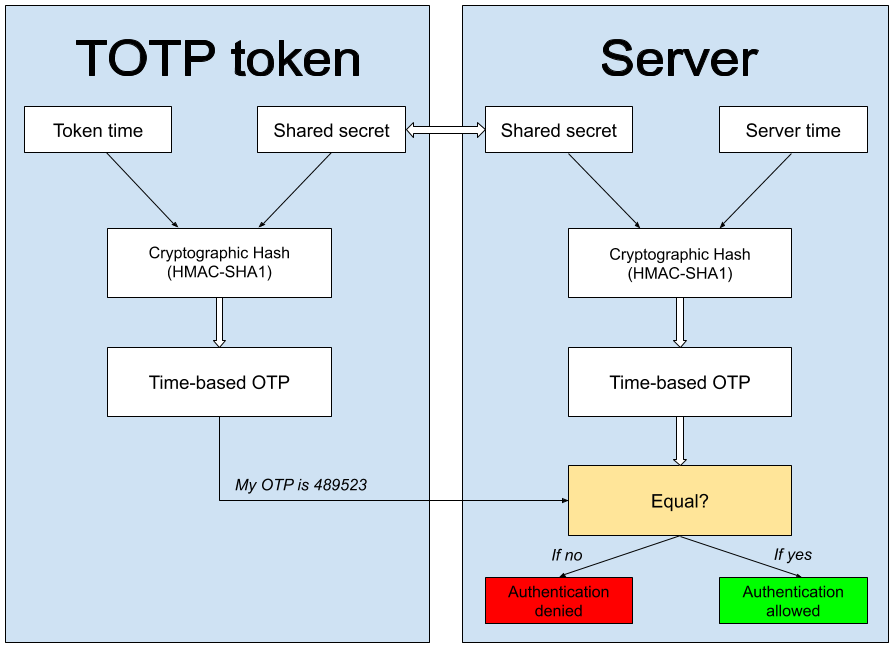
\includegraphics[width=15cm]{TOTP-algorithm-explained.png} \\\\
Bei der timerbasierten (\ac{totp}) Methode wird die aktuelle Systemzeit (Token time) mit dem zu verschlüsselnden Text (Shared secret) anhand eines kryptografischen Verfahrens verschlüsselt. Es entsteht ein kryptografischer Hashwert (Cryptographic Hash), welcher meist den HMAC-SHA1 Hashingalgorithmus verwendet. Dieses Verfahren findet gleichermaßen auf dem Server statt. Der einzige Unterschied zum Server besteht darin, dass die Systemzeit des Servers genutzt wird. Findet innerhalb der festgelegten Zeit (ein Token entfällt laut RFC6238 standartmäßig nach 30 Sekunden, diese Zeit ist modifizierbar) eine erfolgreiche Authentifikation statt, wird der Zugang gewährt. [13]

Ein entscheidender Nachteil dieser Methode entsteht, falls der authentifizierende User innerhalb dieser 30 Sekunden (beispielsweise) durch eine Störung des Netzes oder einen Netzausfall die Verbindung verliert. Der aktuelle TOTP Code wird ungülltig und muss erneut angefragt bzw. erstellt werden. Apps wie der Google Authenticator lösen diesen Problem, in dem sie einen Timer setzen und alle 30 Sekunden einen automatisch generierten neuen Code mit der aktuellen Zeit generieren. Dabei muss natürlich drauf geachtet werden, dass Server und Client synchron sind, dieses Verfahren ist deshalb an eine bestimmte Zeitspanne und ein externes Gerät (sei es Smartphone, TOTP Smart Card oder ein externer Rechner) gebunden.

Laut Margaret Rouse biete das TOTP Verfahren zusätzliche Sicherheit für den Nutzer, da selbst bei Erhalt des Passwortes das TOTP nicht in die Hände des Angreifers gelangt und nach einer gewissen Toleranzzeit verfällt. (\cite{A5} Eine Beispielapplikation für die Nutzung eines TOTP - Ansatzes für zusätzliche Sicherheit ist der "Google Authenticator", welches in jedem gängigen App Store zu finden ist.

Ereignisbasierte OTPs besitzen einen Ereigniszähler, der bei jeder versuchten Authenzifizierung einen Zähler auf Server und Clientseite synchronisiert inkrementiert. Sollte der Zähler asychnron werden bzw. der Server einen anderen Wert gespeichert haben als der Client bei der nächsten Authentifizierung sendet, wird der Authentifizierungsvorgang abgebrochen. Man findet diese Funktionalität wortwörtlich beschrieben in Googles Time and event based one time password" - Patent \cite{A6} in folgendem Wortlaut "[...] the characteristics of an event can be the value of a counter that is incremented each time the user pushes a button on the token" \cite{A6}. Für diesen Prozess wird der HOTP Algorithmus genutzt, der im RFC4226 näher beschrieben ist. Diese Art der Authentifizierung kann zum Beispiel für die E-Mail Verifikation und damit die Identifikation (wie zuvor erläutert) genutzt werden.

Challenge-response basierte OTP Verfahren bedienen sich an komplizierten mathematischen Verfahren. Das heißt, es erfolgt ein ACK (Acknowledge bzw. Initialanstoß zur Authentifizierung). Der Client, berechnet die Response mithilfe der mathematischen Formel und sendet das Ergebnis an den Server. Sollte es einen Match geben, erhält der Client eine Response vom Server, der seine Echtheit bestätigt. Synchronisationsprobleme kann es bei diesem Verfahren entgegen der ereignis oder timerbasierten OTP-Verfahren nicht geben, da die Berechnung dieses 'Schlüssels' vollkommen auf der Clientseite funktioniert. Der Server überprüft diese Rechnung nur mit seinem eigenen Wert, stellt aber keine weiteren Rechnungen oder Umformungen mit diesem Wert an. Der Hauptvorteil dieses Verfahrens ist, dass unabhängig von der Zeit und einem speziellen Ereignis eine Anfrage gestellt werden kann. Der Server kann also seine 'Challenge' abschicken und muss keine 'Response' innerhalb einer festgegebenen Zeit erhalten, um authentifizieren zu können. Dieses Verfahren gilt als besonders sicher, da es auf Serverseite keinen Algorithmus gibt, der sich vorausberechnen lässt.

\subsection{Web Authentication}
Webauthn ist kurz für die 'Web Authentication'. Zur Verfügung gestellt wurde dieser Standard der Authentifikation 2018 von der FIDO Alliance und dem W3C. \cite{A7} Sie ermöglicht eine passwortlose (bzw. benutzerdatenlose, es wird also auch keine User-ID benötigt) Authentifikation durch Tokens (Sicherheitsschlüssel). Für dieses Verfahren wird zunächst ein Buffer aus kryptografischen random Bytes generiert, dass der Verhinderung von 'Bruteforce' (vom webauthn - Guide auch als 'reply attacks' beschrieben) - Angriffen dienen soll. Web Authentication nutzt das vorhandene public-key-Verfahren für Webseiten. Der Standard definiert allerdings nicht welche Art von Schlüssel genutzt wird. Unter den Möglichkeiten zählen der "USB security key" \cite{A7} oder der "built-in fingerprint sensor" \cite{A7}. Webauthn basiert auf vielen bereits vorhandenen Abhängigkeiten der Informatik wie die Standards von HTML5, ECMAScript, COSE (CBOR Object Signing and Encryption COSE, RFC8152) oder dem Nutzen von der Base64url encoding. \\
Zusammengefasst hat der FIDO2 Standard mit CTAP (dem Protokoll für externe Authentifikationen mit Mobilgeräten) und Webauthn (der Schnittstelle bzw. "API") vorhandene Funktionen definiert, mit der native Authentifizierungsmethoden wie das public-private Key Verfahren auf die Webseite übertragen werden können. Wichtige Beispiele für Web Authentication sind der Yubikey, der USB-Token oder unsere biometrischen Daten (FaceID oder TouchID), die wir täglich in jedem AppStore nutzen, der diese Daten verschlüsselt an eine Webseite bzw. einen öffentlichen Store übermittelt. In unserem Use-Case wollen wir die Authentifizierung anhand von Webauthn als Multi-Faktor nutzen, also als zusätzliche Sicherung neben einem Passwort. Denn wie oben beschrieben, kann das Wissen eines Menschen durch Data Breaches oder menschliches Versagen (Gutglauben) leicht abhanden kommen. Mit einem Yubikey oder einem USB-Token befindet man sich allerdings auf der Ebene des Besitzes, wodurch ein potenzieller Angreifer es schwerer hat an die Daten zu kommen. Biometrische Daten und diese public-private-Key Verfahren gelten nämlich allgemein als sehr sicher. Wodurch es technisch sehr schwer bis mathematisch (in gegebener Menschenzeit) fast unmöglich ist, die Algorithmen hinter ihnen zu knacken.
